\section{Towards Capturing Large-Scale Dependencies}\label{sec:towards_large_scale}

In this section, we investigate the ability of graph coupling to faithfully represent the global structure in low dimensions. To gain intuition on the case where the distribution induced by the graph is not degenerate, we consider a proper Gaussian graph coupling model and show its equivalence with PCA. We then provide a new initialization procedure to alleviate the large-scale deficiency of graph coupling when degenerate MRFs are used.

\subsection{Hierarchical Graph Coupling}\label{sec:hierarchical_modelling}

The goal of this section is to show that global structure in SNE-like embeddings can be improved by structuring the CCs' positions. We consider the following hierarchical model for $\Xb$, where $\mathcal{P}_{X} \in \{B,D,E\}$, $k_x$ satisfies the assumptions of \cref{prop:integrability_pairwise_MRF} and $\nu_{X} \geq n$:
\begin{align*}
    \Wb_{X} \sim \mathbb{P}_{\mathcal{P}_X,k_x}^{\varepsilon}(\cdot \: ; \bm{1},1), &\quad \bm{\Theta}_{X} | \Wb_{X} \sim \mathcal{W}(\nu_{X}, \bm{I}_{R}) \\
    \Xb_{C} |\Wb_{X} \sim \mathbb{P}_{k_x}(\cdot \:| \Wb_{X}), &\quad \mathrm{vec}(\Xb_{M}) | \bm{\Theta}_{X} \sim \mathcal{N}\left(\bm{0}, \left(\varepsilon \Ub_{[:R]}  \bm{\Theta}_{X}\Ub^\top_{[R]}\right)^{-1} \otimes \bm{I}_p\right)
\end{align*}
where $\Ub_{R}$ are the eigenvectors associated to the Laplacian null-space of $\overline{\Wb}_{X}$. Given a graph $\Wb_{X}$, the idea is to structure the CCs' relative positions with a full-rank Gaussian model.
The same model is considered for $\Wb_{Z}$, $\bm{\Theta}_{Z}$ and $\Zb$, choosing $\nu_{Z} = \nu_{X} + p - q$ for the Wishart prior to satisfy the assumption of \cref{PCA_graph_coupling}.  With this in place, we aim at providing a complete coupling objective, matching the pairs  $(\Wb_{X},\bm{\Theta}_{X})$ and  $(\Wb_{Z},\bm{\Theta}_{Z})$. The joint negative cross-entropy can be decomposed as follows:
\begin{align}
    &\mathbb{E}_{(\Wb_{X}, \bm{\Theta}_{X})|\Xb}\left[\log \mathbb{P}((\Wb_{Z},\bm{\Theta}_{Z}) = (\Wb_{X},\bm{\Theta}_{X}) | \Zb)\right] \nonumber\\
    &= \mathbb{E}_{\Wb_{X}|\Xb}\left[\log \mathbb{P}(\Wb_{Z} = \Wb_{X} | \Zb)\right] + \label{eq:loss_LW} \\
    & \mathbb{E}_{(\Wb_{X},\bm{\Theta}_{X})|\Xb}\left[ \log \mathbb{P}(\bm{\Theta}_{Z} = \bm{\Theta}_{X}| \Wb_{Z} = \Wb_{X}, \Zb) \right] \label{eq:add_term_Coupling}
\end{align}
where (\ref{eq:loss_LW}) is the usual coupling criterion of $\Wb_X$ and $\Wb_Z$ capturing intra-CC variability while (\ref{eq:add_term_Coupling}) is a penalty resulting from the Gaussian structure on $\mathcal{S}_{M}$. Constructed as such, the above objective allows a trade-off between local and global structure preservation. Following current trends in DR \cite{kobak2021initialization}, we propose to take care of the global structure first \textit{i.e.}\ focusing on (\ref{eq:add_term_Coupling}) before (\ref{eq:loss_LW}). The difficulty of dealing with (\ref{eq:add_term_Coupling}) lies in the hierarchical construction of the graph and the Gaussian precision (see \cref{fig:graphical_model_hierarchical}). We state the following result.

% \begin{wrapfigure}[15]{R}{0.5\textwidth}
% \begin{center}
% \centerline{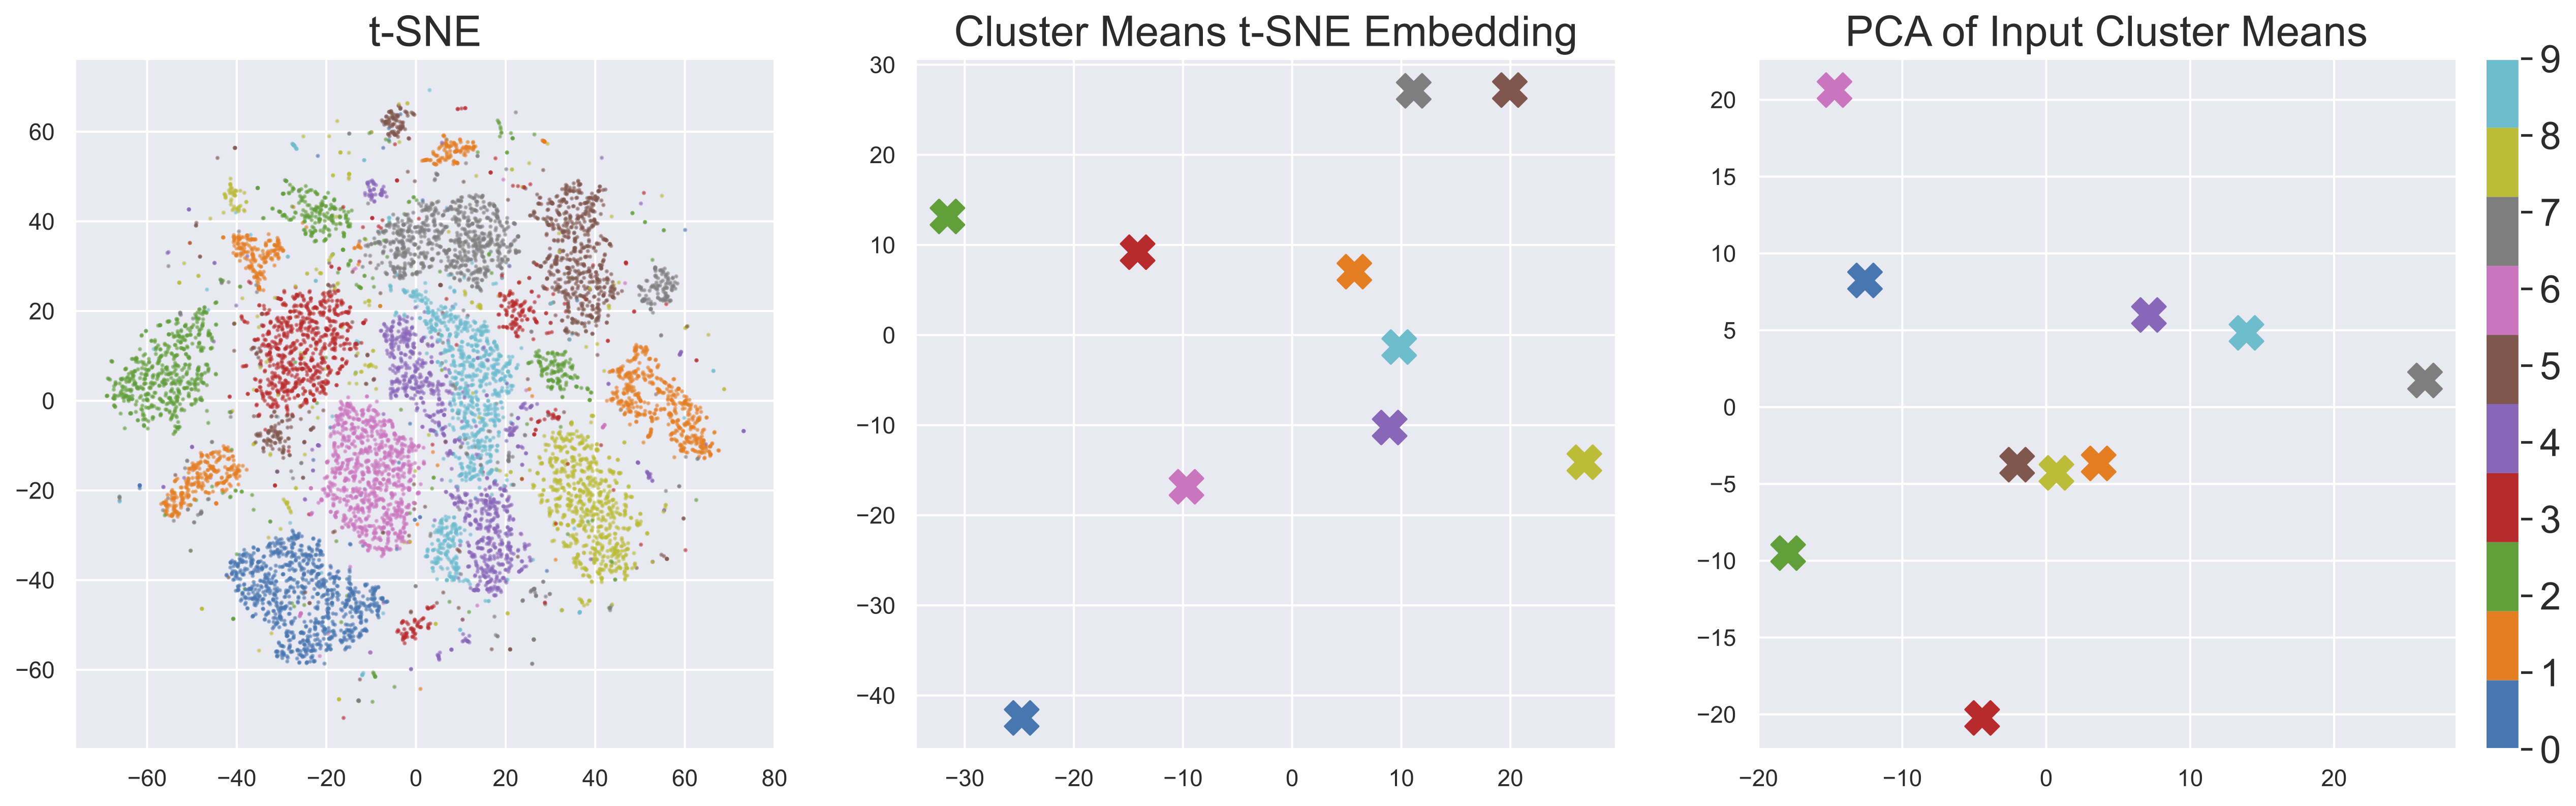
\includegraphics[width=0.5\columnwidth]{figures/GraphCoupling/tSNE_truth.png}}
% \caption{Left: MNIST t-SNE (perp: 30) embeddings initialized with i.i.d $\mathcal{N}(0,1)$ coordinates. Middle: using these t-SNE embeddings, mean coordinates for each digit are represented. Right: we compute a matrix of mean input coordinates for each of the $10$ digits and embed it using PCA. For t-SNE embeddings, the positions of clusters vary across different runs and don't visually match the PCA embeddings of input mean vectors (right plot).}
% \label{fig:tSNE-clusters-truth}
% \end{center}
% \end{wrapfigure}

\begin{corollary}\label{corollary_ccPCA}
Let $\Wb_{X} \in \mathcal{S}_{W}$, $\bm{L} = L(\overline{\Wb}_{X})$ and $\mathcal{S}^q_{M}= (\ker \bm{L}) \otimes \mathbb{R}^q$, then for all $\varepsilon > 0$, given the above hierarchical model, the solution of the problem:
$$\min_{\Zb \in \mathcal{S}^q_{M}} \: -\mathbb{E}_{\bm{\Theta}_{X}| \Xb}\left[ \log \mathbb{P}(\bm{\Theta}_{Z} = \bm{\Theta}_{X}| \Wb_{Z} = \Wb_{X}, \Zb) \right]$$
is a PCA embedding of $\Ub_{[:R]}\Ub_{[R]}^\top\Xb$ where $\Ub_{[:R]}$ are the CCs' membership vectors of $\overline{\Wb}_{X}$.
\end{corollary}

\begin{remark}
Note that while (\ref{eq:loss_LW}) approximates the objective of SNE-like methods when $\varepsilon \to 0$, the minimizer of (\ref{eq:add_term_Coupling}) given by \cref{corollary_ccPCA} is stable for all $\varepsilon$.
\end{remark}

From this observation, we propose a simple heuristic to minimize (\ref{eq:add_term_Coupling}) that consists in computing a PCA embedding of $\mathbb{E}_{\mathbb{P}_{\mathcal{P}_X}(\cdot;\Kb_{X})}\left[ \Ub_{[:R]}\Ub_{[R]}^\top \right]\Xb$. The distribution of the connected components of the posterior of $\Wb_{X}$ being intractable, we resort to a Monte-Carlo estimation of the above expectation. The latter procedure called \textit{ccPCA} aims at recovering the inter-CC structure that is filtered by SNE-like methods. \textit{ccPCA} may then be used as initialization for optimizing (\ref{eq:loss_LW}) which is done by running the DR method corresponding to the graph priors at hand (\cref{sec:retrieving_DR_methods}). This second step essentially consists in refining the intra-CC structure. 

\subsection{Experiments with \textit{ccPCA}}\label{sec:ccPCA}

% \begin{figure*}[t]
% \begin{center}
% \centerline{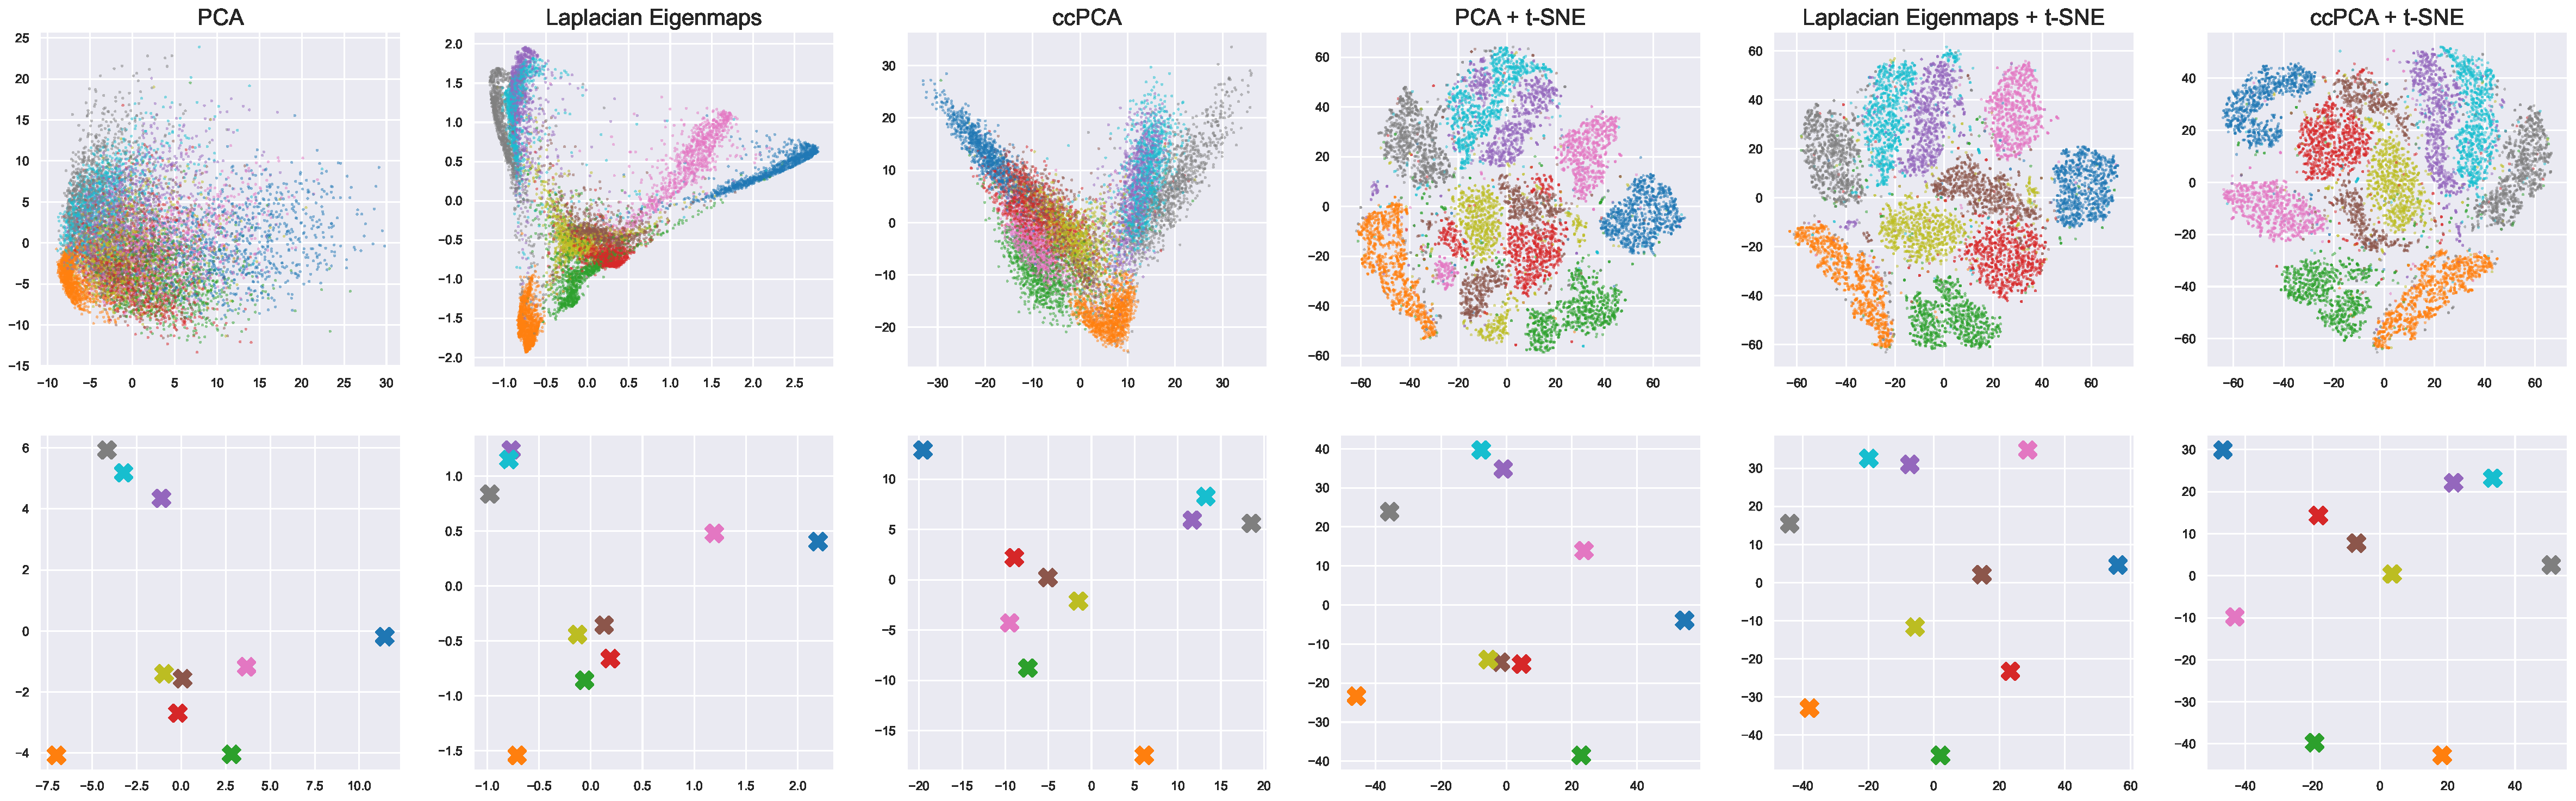
\includegraphics[width=\columnwidth]{figures/GraphCoupling/cluster_positions.png}}
% \caption{Top: MNIST embeddings produced by PCA, Laplacian eigenmaps, \textit{ccPCA} and finally t-SNE launched after the previous three embeddings to improve the fine-grain structure. Bottom: mean coordinates for each digit using the embeddings of the first row. The color legend is the same as in \cref{fig:tSNE-clusters-truth}. t-SNE was trained during $1000$ iterations using default parameters with the openTSNE implementation \cite{polivcar2019opentsne}.}
% \label{fig:methods_embeddings}
% \end{center}
% \vspace{-0.8cm}
% \end{figure*}

\Cref{fig:tSNE-clusters-truth} shows that a t-SNE embedding of a balanced MNIST dataset of 10000 samples \cite{deng2012mnist} with isotropic Gaussian initialization performs poorly in conserving the relative positions of clusters. As each digit cluster contains approximately $1000$ points, with a perplexity of $30$, sampling an edge across digit clusters in the graph posterior $\mathbb{P}_{\mathcal{P}_X}(\cdot;\Kb_{X})$ is very unlikely. Recall that the perplexity value \cite{maaten2008tSNE} corresponds to the approximate number of effective neighbors of each point. Hence images of different digits are with very high probability in different CCs of the graph posterior and their CC-wise means are not coupled as discussed in \cref{sec:interpretations}. To remedy this in practice, PCA or Laplacian eigenmaps are usually used as initialization \cite{kobak2021initialization}. 

These strategies are tested (\cref{fig:methods_embeddings}) together with \textit{ccPCA}. This shows that 
\textit{ccPCA} manages to retrieve the digits that mostly support the large-scale variability as measured by the peripheral positioning of digits $0$ (blue), $2$ (green), $6$ (pink) and $7$ (grey) given by the right side of \cref{fig:tSNE-clusters-truth}. Other perplexity values for \textit{ccPCA} are explored in appendix \ref{sec:other_perp} while the experimental setup is detailed in appendix \ref{sec:setup_exp}. In appendix \ref{sec:quantitative_evaluation}, we perform quantitative evaluations of \textit{ccPCA} for both t-SNE and UMAP on various datasets using K-ary neighborhood criteria. We find that using \textit{ccPCA} as initialization is in general more reliable than PCA and Laplacian eigenmaps for preserving global structure using both t-SNE and UMAP. 

Compared to PCA, \textit{ccPCA} manages to aggregate points into clusters, thus filtering the intra-cluster variability and focusing solely on the inter-cluster structure. Compared to Laplacian eigenmaps which perform well at identifying clusters but suffer from the same deficiency as t-SNE for positioning them, \textit{ccPCA} retains more of the coarse-grain structure. These observations support our unifying probabilistic framework and the theoretical results about the MRF degeneracy which are the leading contributions of this article. The \textit{ccPCA} initialization appears as a first stepping stone towards more grounded DR methods based on the probabilistic model presented in this article.